\documentclass[aspectratio=169]{beamer}

\mode<presentation>
{
  \usetheme{Warsaw}
  % or ...

  \setbeamercovered{transparent}
  % or whatever (possibly just delete it)
}


\usepackage[english]{babel}
\usepackage[latin1]{inputenc}
\usepackage{graphicx}
%\usepackage{times}
%\usepackage[T1]{fontenc}
% Or whatever. Note that the encoding and the font should match. If T1
% does not look nice, try deleting the line with the fontenc.

\usepackage{amsmath,amsfonts,amssymb}

\newcommand{\pkg}{\textbf}
\newcommand{\code}{\texttt}


\title[Simulation]{Simulation}


\date{Computing for Data Analysis}



\begin{document}

\begin{frame}
  \titlepage
\end{frame}

\begin{frame}{Generating Random Numbers}
  Functions for probability distributions in R
\begin{itemize}
  \item \code{rnorm}: generate random Normal variates with a
    given mean and standard deviation
  \item \code{dnorm}: evaluate the Normal probability density (with a
    given mean/SD) at a point (or vector of points)
  \item \code{pnorm}: evaluate the cumulative distribution function
    for a Normal distribution
  \item \code{rpois}: generate random Poisson variates with a given
    rate
\end{itemize}
\end{frame}


\begin{frame}{Generating Random Numbers}
  Probability distribution functions usually have four functions
  associated with them. The functions are prefixed with a
\begin{itemize}
\item \code{d} for density
\item \code{r} for random number generation
\item \code{p} for cumulative distribution
\item \code{q} for quantile function
\end{itemize}
\end{frame}


\begin{frame}[fragile]{Generating Random Numbers}
Working with the Normal distributions requires using these four
functions
\begin{verbatim}
dnorm(x, mean = 0, sd = 1, log = FALSE)
pnorm(q, mean = 0, sd = 1, lower.tail = TRUE, log.p = FALSE)
qnorm(p, mean = 0, sd = 1, lower.tail = TRUE, log.p = FALSE)
rnorm(n, mean = 0, sd = 1)
\end{verbatim}
If $\Phi$ is the cumulative distribution function for a standard
Normal distribution, then $\text{\code{pnorm}}(q) = \Phi(q)$ and
$\text{\code{qnorm}(p)} = \Phi^{-1}(p)$.
\end{frame}

\begin{frame}[fragile]{Generating Random Numbers}
Generating random Normal variates
\begin{verbatim}
> x <- rnorm(10)
> x
 [1] 1.38380206 0.48772671 0.53403109 0.66721944
 [5] 0.01585029 0.37945986 1.31096736 0.55330472
 [9] 1.22090852 0.45236742
> x <- rnorm(10, 20, 2)
> x
 [1] 23.38812 20.16846 21.87999 20.73813 19.59020
 [6] 18.73439 18.31721 22.51748 20.36966 21.04371
> summary(x)
   Min. 1st Qu.  Median    Mean 3rd Qu.    Max. 
  18.32   19.73   20.55   20.67   21.67   23.39 
\end{verbatim}
\end{frame}

\begin{frame}[fragile]{Generating Random Numbers}
Setting the random number seed with \code{set.seed} ensures
reproducibility
\begin{verbatim}
> set.seed(1)
> rnorm(5)
[1] -0.6264538  0.1836433 -0.8356286  1.5952808
[5]  0.3295078
> rnorm(5)
[1] -0.8204684  0.4874291  0.7383247  0.5757814
[5] -0.3053884
> set.seed(1)
> rnorm(5)
[1] -0.6264538  0.1836433 -0.8356286  1.5952808
[5]  0.3295078
\end{verbatim}
Always set the random number seed when conducting a simulation!
\end{frame}

\begin{frame}[fragile]{Generating Random Numbers}
Generating Poisson data
\begin{verbatim}
> rpois(10, 1)
 [1] 3 1 0 1 0 0 1 0 1 1
> rpois(10, 2)
 [1] 6 2 2 1 3 2 2 1 1 2
> rpois(10, 20)
 [1] 20 11 21 20 20 21 17 15 24 20

> ppois(2, 2)  ## Cumulative distribution
[1] 0.6766764  ## Pr(x <= 2)
> ppois(4, 2)
[1] 0.947347   ## Pr(x <= 4)
> ppois(6, 2)
[1] 0.9954662  ## Pr(x <= 6)
\end{verbatim}
\end{frame}

\begin{frame}[fragile]{Generating Random Numbers From a Linear Model}
Suppose we want to simulate from the following linear model
\[
y = \beta_0 + \beta_1 x + \varepsilon
\]
where $\varepsilon\sim\mathcal{N}(0, 2^2)$. Assume
$x\sim\mathcal{N}(0,1^2)$, $\beta_0 = 0.5$ and $\beta_1 = 2$.
\begin{verbatim}
> set.seed(20)
> x <- rnorm(100)
> e <- rnorm(100, 0, 2)
> y <- 0.5 + 2 * x + e
> summary(y)
   Min. 1st Qu.  Median    Mean 3rd Qu.    Max. 
-6.4080 -1.5400  0.6789  0.6893  2.9300  6.5050 
> plot(x, y)
\end{verbatim}
\end{frame}

\begin{frame}[fragile]{Generating Random Numbers From a Linear Model}
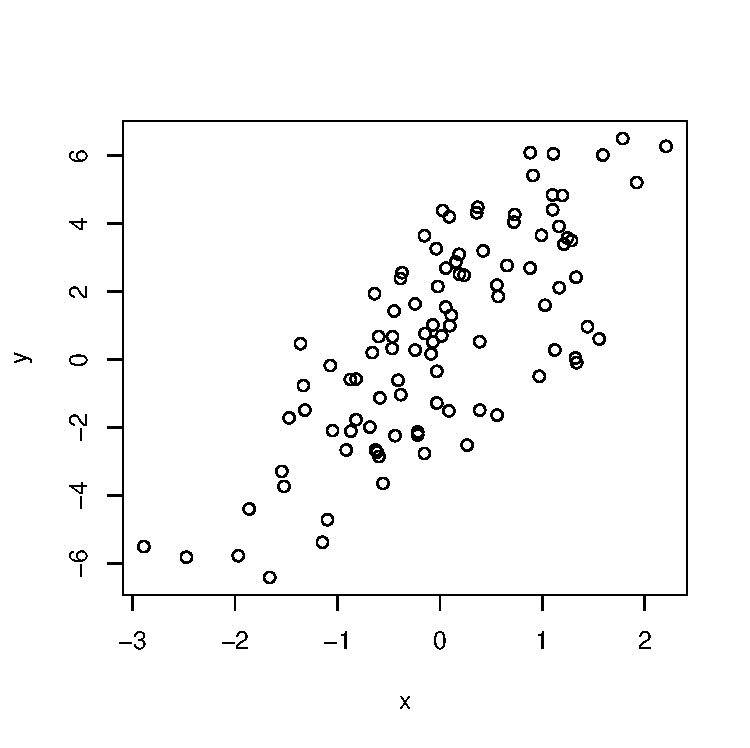
\includegraphics[height=3.2in]{linearmodelsim}
\end{frame}

\begin{frame}[fragile]{Generating Random Numbers From a Linear Model}
What if \code{x} is binary?
\begin{verbatim}
> set.seed(10)
> x <- rbinom(100, 1, 0.5)
> e <- rnorm(100, 0, 2)
> y <- 0.5 + 2 * x + e
> summary(y)
   Min. 1st Qu.  Median    Mean 3rd Qu.    Max. 
-3.4940 -0.1409  1.5770  1.4320  2.8400  6.9410 
> plot(x, y)
\end{verbatim}
\end{frame}

\begin{frame}[fragile]{Generating Random Numbers From a Linear Model}
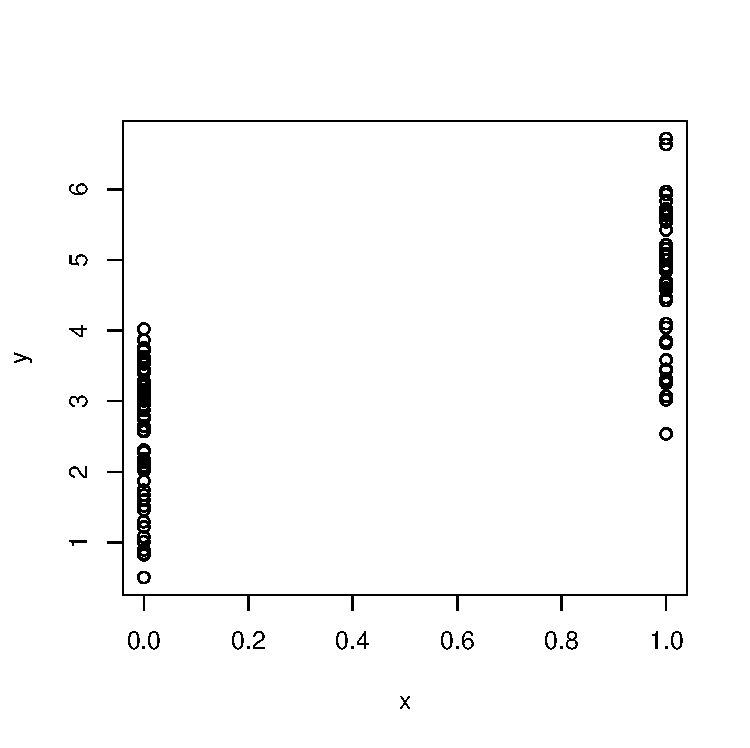
\includegraphics[height=3.2in]{binarylinearmodelsim}
\end{frame}

\begin{frame}[fragile]{Generating Random Numbers From a Generalized
    Linear Model}
Suppose we want to simulate from a Poisson model where
\begin{eqnarray*}
Y & \sim & \text{Poisson}(\mu)\\
\log\mu & = & \beta_0 + \beta_1 x
\end{eqnarray*}
and $\beta_0 = 0.5$ and $\beta_1 = 0.3$.  We need to use the
\code{rpois} function for this
\begin{verbatim}
> set.seed(1)
> x <- rnorm(100)
> log.mu <- 0.5 + 0.3 * x
> y <- rpois(100, exp(log.mu))
> summary(y)
   Min. 1st Qu.  Median    Mean 3rd Qu.    Max. 
   0.00    1.00    1.00    1.55    2.00    6.00 
> plot(x, y)
\end{verbatim}
\end{frame}

\begin{frame}[fragile]{Generating Random Numbers From a Generalized Linear Model}
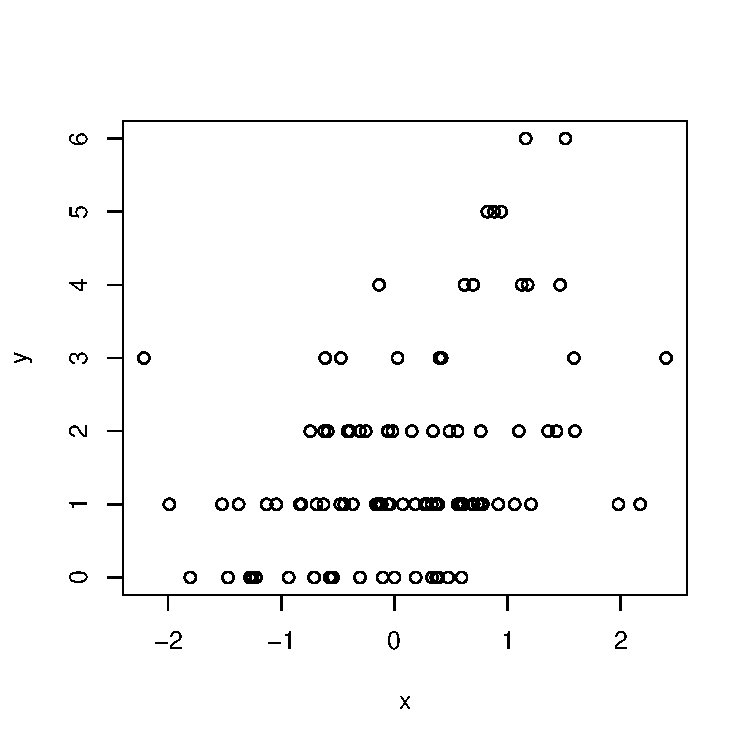
\includegraphics[height=3.2in]{simpoisson}
\end{frame}

\begin{frame}[fragile]{Random Sampling}
  The \code{sample} function draws randomly from a specified set of
  (scalar) objects allowing you to sample from arbitrary
  distributions.
\begin{verbatim}
> set.seed(1)
> sample(1:10, 4)
[1] 3 4 5 7
> sample(1:10, 4)
[1] 3 9 8 5
> sample(letters, 5)
[1] "q" "b" "e" "x" "p"
> sample(1:10)  ## permutation
 [1]  4  7 10  6  9  2  8  3  1  5
> sample(1:10)
 [1]  2  3  4  1  9  5 10  8  6  7
> sample(1:10, replace = TRUE)  ## Sample w/replacement
 [1] 2 9 7 8 2 8 5 9 7 8
\end{verbatim}
\end{frame}

\begin{frame}{Simulation}
Summary
\begin{itemize}
\item Drawing samples from specific probability distributions can be
  done with \code{r}* functions
\item Standard distributions are built in: Normal, Poisson, Binomial,
  Exponential, Gamma, etc.
\item The \code{sample} function can be used to draw random samples
  from arbitrary vectors
\item Setting the random number generator seed via \code{set.seed} is
  critical for reproducibility
\end{itemize}
\end{frame}

\end{document}


